\documentclass[a4paper,12pt]{article}
    \usepackage{amsmath}
    \usepackage{amsfonts}
    \usepackage[utf8]{inputenc}
    \usepackage{titlepic}
    \usepackage{stackengine}
    \usepackage{lipsum}
    \usepackage{graphicx}
    \usepackage{booktabs}
    \usepackage{cite}
	\usepackage{caption}
	\usepackage{float}
	\usepackage{subcaption}
    \usepackage{multirow}
    \usepackage[top=1in, bottom=1in, left=1in, right=1in]{geometry}
    \usepackage{fancyhdr}
    \usepackage{relsize}
    \usepackage{tikz}
    \usetikzlibrary{shapes.geometric,arrows}
	\makeatletter
    \setlength{\@fptop}{0pt}
    \makeatother
    \tikzstyle{startstop} = [rectangle, rounded corners, minimum width = 4cm, minimum height=1cm, text centered, draw = black, fill=blue!10]    
     \tikzstyle{process} = [rectangle,  minimum width = 4cm, minimum height=1cm, text centered, text width = 4cm,draw = black, fill = blue!10]  
	 \tikzstyle{decision} = [diamond, minimum width = 4cm, minimum height=1cm, text centered, draw = black, fill = blue!10]  
     \tikzstyle{arrow} = [thick,->,>=stealth]  


\usepackage{titling}
\pretitle{\begin{center}\fontsize{18bp}{18bp}\selectfont}
    \posttitle{\vspace{25bp}\par
\includegraphics[width=60mm]{logo.png}\par\end{center}}
\preauthor{\begin{center}\fontsize{14bp}{14bp}\selectfont}
    \postauthor{\par\end{center}}
\predate{\begin{center}}
    \postdate{\par\end{center}}  

\title{\Huge{\textbf{Development and implementation of material subroutine for fibre reinforced plastics in a commercial FEM software}}\\[1.3cm]\smaller \textbf{Master thesis \\[0.5cm] Winter semester 2018/19}\vspace*{1cm}}


\author{
\vspace{2cm}
\Large{Presented by: Arun prakash Ganapathy}
\\[0.4cm]
\Large{Supervised by: Dr.-Ing Dominik Laveuve}
\\[0.4cm]
\Large{Mat.Nr: 63876}
\\[0.4cm]
\Large{E-mail: arun-prakash.ganapathy@student.tu-freiberg.de}}
\date{}

\begin{document}
\maketitle
\section{Introduction}
\subsection{Background and motivation}
\indent\indent Composite materials are made of two or more dissimilar materials of different physical or chemical properties when combined, create a material with properties unlike the individual constituent materials. The earliest use of composite materials date back to 3400 B.C when Mesopotamians glued wood strips at different angles to create plywood. Another notable example is the bow made by Mongols during 1200 A.D, which is made from a combination of bamboo, wood, cattle tendons and silk bonded with natural resin. In the early, 1900s bakelite based composites were developed for its non-conductivity and heat resistant properties and widely used in industrial and consumer applications. Now a days advanced composite materials are widely used in structural design in various industries such as aerospace, automobile, marine, petrochemical etc., due to their superior properties over traditional engineering materials.\\
\begin{figure}[htbp]
\begin{center}
\includegraphics[width=0.8\textwidth]{{composite plane.jpg}}
 \caption{Composite materials used in a Boeing 787 'Dreamliner'}
 \label{fig:Composite plane}
\end{center}
\end{figure}\\
 Composite material are attractive because of their high strength, stiffness, high stiffness-to-density ratio, light weight properties etc., Another important reason for using composite materials is the ability to tailor the stiffness and strength to specific design load flexibly. Despite their superior physical properties, composite materials are fragile and can be easily damaged from number of sources, both during initial processing and in operation. Since composite materials possess elastic brittle properties with negligible margin of safety through ductility as offered by metals and accumulate damage before structural collapse, the development of damage must be understood for predicting failure of such materials. For example fibre-reinforced plastics exhibit local damage such as fibre breakage, matrix cracks, fibre matrix debonds etc., under normal operating conditions which may contribute to the failure. Therefore the ability to predict the initiation and growth of damage is important for predicting the performance of the composite materials for safe and reliable use of such materials. Continuum damage mechanics (CDM) has been considered as a reliable candidate for creating numerical models which predict the onset and evolution of the damage in the composite materials.
\section{Continuum damage mechanics}
\indent\indent\indent Continuum damage mechanics (CDM) is a theory for analyzing damage and fracture processes in materials from continuum mechanics point of view. Continuum damage mechanics (CDM) provides a continuum perspective for microflaws initiation, propagation, and their coalescence that eventually results in macroscopic faults and fractures. CDM uses state variables to represent the effect of damage on the stiffness and remaining life of the material that is damaging as a result of load and ageing. A Damage activation function is required to predict the initiation of damage. Damage evolution does not progress spontaneously after initiation therefore a mathematical model is required.  In plasticity formulations, the damage evolution is controlled by a hardening function but this requires additional phenomenological parameters that must be found through experimentation, which is expensive and time consuming. On the other hand, micromechanics of damage formulations are able to predict both damage initiation and evolution without additional material properties.
\subsection{Damage}
\indent\indent\indent  Consider a body B of Fig. \ref{fig:Damage}  where a crack of length a has developed due to an external load F.  If we take an arbitrary point P($x$) near the crack tip, a number of microscopic cavities or microcracks would be observed around the region.
These cavities can be nucleated usually as a result of breakage of atomic bonds, or of some defects in atomic array. From microscopic point of view, fracture of materials is a process of nucleation of microcavities or microcracks due to the breakage of atomic bonds. From macroscopic point of view, it is a process of extension of cracks brought about by the coalescence of these microcracks. From mesoscopic point of view, which exists between microscopic and macroscopic scale, it is a process of nucleation, growth and the coalescence of microscopic cavities leads to the initiation of macroscopic crack. The development of microscopic, mesoscopic and the macroscopic processes of fracture in materials together with the resulting deterioration in their mechanical properties is called damage. Continuum damage mechanics, in particular, aims at the analysis of the damage development in mesoscopic and macroscopic fracture processes in the framework of continuum mechanics.
\begin{figure}[htbp]
\begin{center}
\includegraphics[width=0.4\textwidth]{{1. Damage.png}}
 \caption{Scales of damage observation}
 \label{fig:Damage}
\end{center}
\end{figure}
\newpage
The seperation of atomic bonds is induced either by shear or tensile decohesion. However the separation of material at the microscopic level consists of four damage mechanisms namely Cleavage, Growth and Coalescence of Microvoids, Glide plane decohesion and Void Growth due to Grain-Boundary diffusion.  The aspects of damage vary largely by difference in materials and loading conditions. The damage may be classified phenomenologically as follows
\begin{itemize}
\item Ductile Damage
\item Brittle Damage
\item Creep Damage
\item Low Cycle Fatigue
\item Very Low Cycle Fatigue
\item High Cycle fatigue damage
\item Very High Cycle fatigue damage
\item Creep Damage
\end{itemize}
\subsection{Representative Volume Element(RVE)}
\indent\indent\indent  In order to discuss the effects of microscopic discontinuities in  a material by means of CDM we must homogenize the mechanical effects of microstructure and represent them as a macroscopic continuous field in the material. For this purpose we take a small region of a mesoscale around the material point P($x$) in a body B as showin in Fig. \ref{fig:Damage}. We assume that the  material with discontinuous structures in this region can be statistically homogeneous and the mechanical state of the material in this region can be represented by the statistical average of the mechanical variables in that region. This region is said to be the Representative Volume Element(RVE). For such RVE, the following two conditions must be satisfied:
\begin{itemize}
\item  For the material in the RVE to be statistically homogeneous, the RVE should be large enough to contain a sufficient number of discontinuities
\item In order to represent a non-uniform macroscopic mechanical field by means of a continuum, the size of RVE should be sufficiently small so that the variation of the macroscopic variable in it may be insignificantly small
\end{itemize}
The size of RVE depends on the microstructure of the relevant material and their typical sizes are as follows
\begin{itemize}
\item Metals and ceramics  \;    -    \; 0.1$mm^3$
\item Polymer and composites \;   -   \; 1$mm^3$
\item Timber\; - \; 10$mm^3$
\item Concrete \; - \; 100$mm^3$
\end{itemize}
\newpage
\subsection{Concept of Continuum damage mechanics (CDM)}
\indent\indent\indent The basic concept of CDM is to that microstructural defects in a material can be represented by a set of damage variables.  Continuum damage mechanics first represent the damage state of a material in terms of damage variables and then describe the mechanical behaviour of the damaged material and then development of damage by use of these damage variables.
Let us consider a body B of Fig. \ref{fig:Damage2} and take a representative volume element(RVE) at an arbitrary point $P(x)$ in B. If the total void area in $dA$ is  $ dA_{D} $, the mechanical effect of $dA$ will be decreased by $dA_{D}$. Then the area,
\begin{equation}
  d\tilde{A} = dA  - dA_{D} 
\end{equation}
may be interpreted as the area which carries the internal force and is called as $effective area$. Thus the damage variable D can be specified as 
\begin{equation}
  D = \frac{dA - d\tilde{A}}{dA} = \frac{dA_{D}}{dA}
\end{equation}
where the damage variable D takes value between 0 and 1 ($0 \leq D \leq 1$). $D = 0$ representing initial undamaged state and $D=1$ represents fully damaged state.
\begin{figure}[htbp]
\begin{center}
\includegraphics[width=0.8\textwidth]{{Damage2.png}}
 \caption{Effective area reduction due to microcracks}
 \label{fig:Damage2}
 \end{center}
\end{figure}
Suppose a cylindrical bar of cross-sectional area $dA$ is subject to a tensile load $dF$ the actual load carrying area is $ d\tilde{A}$ rather than $dA$. According to eqn (1) and (2) the effective area $ d\tilde{A}$ is given by,
\begin{equation}
 d\tilde{A} = (1-D)dA
\end{equation}
The decrease in load-carrying area increase the effect of stress $\sigma$ induced by the external force $dF$. Due to eqn (3) the magnified stress $\tilde{\sigma}$ is given by,
\begin{equation}
\tilde{\sigma} = \frac{dF}{d\tilde{A}} = \frac{\sigma}{1 - D}
\end{equation} 
\newpage
Since the stress $\tilde{\sigma}$ represents the effect of stress magnified by the net area reduction due to damage, it is called as effective stress. From eqn (3) and (4) we can postulate that the damaged cylindrical bar of Fig.\ref{fig:Damage3}b with the cross-section $dA$ subject to force $dF$ is mechanically equivalent to the fictious undamaged bar of Fig.\ref{fig:Damage3}c which is subject to force $dF$ , has the cross-section $ {d\tilde{A}} $ and hence stress has the stress $\tilde{\sigma}$  
\begin{figure}[htbp]
\begin{center}
\includegraphics[width=0.8\textwidth]{{3. Damage_cylinder.png}}
 \caption{Damage of bar under tensile load}
 \label{fig:Damage3}
 \end{center}
\end{figure}

\subsubsection{Modelling by variation of elastic modulus} 
\indent\indent\indent Since the development of microcracks induces the reduction in stiffness of material, the damage state can be characterized by variation in elastic modulus. Let us consider the bar (b) and (c) of Fig\ref{fig:Damage3} are in damaged and fictitious undamaged state respectively. Then the elastic strain $\epsilon$ in the bar (c) caused by stress $\tilde{\sigma}$ should be equal to the $\epsilon$ of the bar (b) under stress $\sigma$; i.e.,\\
\begin{equation}
   \tilde{\sigma} = E_{0}\epsilon, \;\;  \sigma = E(D)\epsilon 
\end{equation}
\\
\begin{equation}
\epsilon = \frac{\sigma}{E(D)} = \frac{\tilde{\sigma}}{E_{0}}
\end{equation}
where $E_{0}$ and $E(D)$ denote young's modulus of the material in the initial undamaged state and that in damaged state after loading, respectively. Therefore, eqn(6) defines another effective stress\\
\begin{equation}
\epsilon = \frac{E_{0}}{E(D)}\sigma
\end{equation}
By combining Eqn(4) and (6) we get,
\begin{equation}
E(D) = (1 - D) E_{0}
\end{equation}
\begin{equation}
D  = 1 - \frac{E(D)}{E_{0}}
\end{equation}
Therefore, the damage variable $D$ is characterized by the variation in Young's modulus $E(D)$. The modelling of damage by means of reduction in stiffness can be applied also the anisotropic damage of brittle materials like composite materials, concrete, rocks etc.,
\subsection{Mechanical representation of three dimensional damage state}
\indent\indent\indent The deformation of a material basically depends on the direction of applied stress or strain and hence it is an anisotropic phenomenon. Therefore different theories have been developed for modelling 3-D anisotropic damage phenomenon. Some fundamental theories that describes 3-D damage state are given below 
\subsubsection*{Scalar Damage Variable}
\indent\indent\indent In case of random or isotropic distribution of microcracks or voids , the damage state is usually considered as isotropic. the damage state in this case may be represented by means of scalar damage variable D. When microvoids  have oriented distribution the damage state is anisotropic and the scalar damage variable cannot be applied accurately. However, when void density is small the global mechanical properties can be approximated as nearly isotropic. thus isotropic damage theory based on isotropic damage variable has been often applied to 3-D problems of creep, elastic-plastic, ductile and fatigue damage
\subsubsection{Plural Scalar damage variables}
\indent\indent\indent A single scalar damage variable is often insufficient to describe the variation in mechanical properties of the damaged materials, even if the distribution of microcracks are isotropic. Plural scalar damage variables are often employed to characterize several different microscopic mechanisms of the relevant damage development.
\subsubsection{Vector damage variable}
\indent\indent\indent The damage state can be specified by the decrease in load carrying effective area due to void development. Hence it is easy to postulate a vector damage variable. Kachanov (1974, 1986) tried to extend the definition of damage to anisotropic damage by noting a surface element in an arbitrary direction $n$, he proposed a vector damage variable $ \omega = \omega_{n}n$, where $\omega_{n}$ is the effective area fraction. However the damage variable $D(n)$ discussed at the beginning representing the damage state of a plane with specific unit normal vector $n$ should be unchanged irrespective of the  change in the sense of $n$ and hence we have the requirement,
\begin{equation}
 D(n) = D(-n)
\end{equation}
\subsubsection{Damage tensor of second order}
\indent\indent\indent In order to describe an anisotropic damage state, damage variable of second or higher order tensor is required. Eqn. (3) suggests that the damage state (1 - D) is specified by the transformation of the surface element $dA$ of Fig. \ref{fig:Damage3}b of the damage state into the corresponding surface element $d\tilde{A}$ in the fictitious undamaged state of Fig. \ref{fig:Damage3}c 
\begin{figure}[htbp]
\begin{center}
\includegraphics[width=0.5\textwidth]{{4. Damage.png}}
 \caption{Surface element in RVE of a damaged material}
 \label{fig:Damage4}
 \end{center}
\end{figure}
In order to express damage as a second order tensor, we first consider an arbitrary surface element $PQR$ in RVE in the current damaged configuration $B_{t}$ of Fig. \ref{fig:Damage4}a . The unit normal vector and area of $PQR$ are denoted by $\nu$ and $dA$. We further postulate the fictitious undamaged configuration $B_{f}$ of Fig. \ref{fig:Damage4}b mechanically equivalent to $B_{t}$, and the surface element and its area vector are denoted by $\tilde{P}\tilde{Q}\tilde{R}$ and $\tilde{\nu}d\tilde{A}$ respectively. According to Eqn.(3) the damage variable of second-order tensor $D$ should be defined by linear transformation from area vector $\nu dA$ in $B_{t}$ into $\tilde{\nu}d\tilde{A}$ in $B_{f}$, i.e.,
\begin{equation}
\tilde{\nu}d\tilde{A} = (I - D)\nu dA
\end{equation}
where $I$ is the second order identity tensor. Since the damage tensor $D$ is symmetric, it can be expressed by its spectral decomposition
\begin{equation}
D = \sum_{i = 1}^{3} D_{i}n_{i}  \otimes D_{i}n_{i}
\end{equation}
where $D_{i}$ and $n_{i}$ are the principal value and principal direction of $D$. 
\subsubsection{Damage tensors of Fourth order and eighth order}
\indent\indent\indent Let us consider the fourth-order elastic modulus tensor of an undamaged and the damaged material be denoted by $\mathbb{C}_{0}$ and $\mathbb{C}(D)$. Then the elastic constitutive equation of these materials is given by \\
\begin{equation}
  \sigma  =  \mathbb{C}_{0} : \epsilon  \;\;\;  \sigma = \mathbb{C}(D) : \epsilon
\end{equation}
where (:) denotes the double contraction. Since the the elastic strain in a damaged material under stress $\sigma$ is equal to the equivalent fictitious undamaged material subject to effective stress $\sigma$, we have
\begin{equation}
 \tilde{\sigma}  = \mathbb{C}_{0} : \epsilon
\end{equation}
Form Eqn (13) and (14) we can represent effective stress as 
\begin{equation}
\tilde{\sigma}  = [\mathbb{C}_{0} : \mathbb{C}(D)^{-1}] : \sigma
\end{equation}
From equation (13), the damage tensor $D$ may be viewed as an eighth-order tensor which transforms fourth order elasticity tensor $\mathbb{C}_{0}$ of an undamaged material into another fourth-order tensor $\mathbb{C}(D)$ of the damaged material. Since mathematical operation of eighth-order tensor is highly complicated an alternative fourth-order damage tensor $\mathbb{D}$ has been proposed and the transformation between elastic moduli is given by,
\begin{equation}
\mathbb{C}(\mathbb{D})  =  (\mathbb{I}  - \mathbb{D}) : \mathbb{C}_{0}
\end{equation}
where $\mathbb{I}$ denotes the fourth-order identity tensor. The fourth order damage tesnor $\mathbb{D}$ and the effecctive stress tensor $\tilde{\sigma}$ are given by the following relations
\begin{equation}
\mathbb{D}  = \mathbb{I} - \mathbb{C}(\mathbb{D}) : \mathbb{C}_{0}^{-1}
\end{equation}\\
\begin{equation}
\tilde{\sigma} =  (\mathbb{I} - \mathbb{D})^{-1} : \sigma
\end{equation}
Since the damage tensor $\mathbb{D}$ given by Eqn(17) is asymmetric, Chaboche(1993) later employed an alternative transformation,
\begin{equation}
\mathbb{C}(\hat{\mathbb{D}}) = \frac{1}{2}\; [(\mathbb{I} - \hat{\mathbb{D}}) : \mathbb{C}_{0} + \mathbb{C}_{0} : (\mathbb{I} - \hat{\mathbb{D}}  ]
\end{equation}
and proposed a new fourth-order symmetric tensor $\hat{\mathbb{D}}$.
\subsection{Effective Stress Tensors}
\indent\indent\indent The effective stresses are  used to describe the mechanical behaviour of the damaged material. Some of the effective stresses postulated in damage mechanics are given below
\subsubsection{Effective Stress Tensor for Isotropic Damage}
\indent\indent\indent If the damage state is isotropic then the effective stress tensor of three-dimensional state is given by
\begin{equation}
\tilde{\sigma} = (1 - D)^{-1} \; \sigma
\end{equation}
where D is the scalar damage variable and $\sigma$ is the Cauchy stress tensor. This effective stress simplifies damage theory and can be applied to number of damage problems like ductile damage. But this cannot be applied to damage of significant anisotropy, such as brittle damage due to microcrack distribution\\
\subsubsection{Asymmetric Effective Stress Tensor for Anisotropic Damage}
\indent\indent\indent The increase in stress effect caused by the net area reduction in case of anisotropic damage is given by
\begin{equation}
\tilde{\sigma} = (I - D)^{-1} \; \sigma
\end{equation}
where I and D are second order identity tensor and the second order damage tensor respectively. In the actual development of anisotropic damage, the stress induced in RVE of damage material is asymmetric. But asymmetric stress tensor makes the numerical analysis complicated and thus different methods of symmetrization has been proposed. Few of them are described as follows
\newpage
\subsubsection{Symmetrized Effective Stress Tensor for Anisotropic Damage 1 (Murakami and Ohno 1981)} 
\indent\indent\indent A simple symmetrization procedure of Eq. (21), the symmetric part of the Cartesian decomposition of Eq. (21) gives,
\begin{equation}
\tilde{\sigma} = \frac{1}{2} [(I - D)^{-1}\;\sigma + \sigma(I - D)^{-1}]
\end{equation}\\
\subsubsection{Symmetrized Effective Stress Tensor for Anisotropic Damage 2 (Cordebois and Sidoroff 1982a, b)}
\indent\indent\indent Another form of symmetrization was proposed by Cordebois and Sidoroff:
\begin{equation}
\tilde{\sigma} =  (I - D)^{-1/2}\sigma(I - D)^{-1/2}
\end{equation}
where $\sigma$ and $D$ are co-axial. Moreover, unless the development of damage is large, the difference between these effective stresses are known to be insignificant.\\
\subsubsection{Symmetrized Effective Stress Tensor for Anisotropic Damage 3 ((Betten 1986)}
\indent\indent\indent  Betten derived another effective stress tensor , ie.,
\begin{equation}
\tilde{\sigma} =  (I - D)^{-1}\sigma(I - D)^{-1}
\end{equation} 
Since tensors $(I - D)^{-1}$ and $(I - D)^{-1/2}$ are both second-order symmetric positive tensor, there is no essential difference between Eqs. (23) and (24).

\subsection{Matrix Representation of Damage effect tensors}
\indent\indent\indent The general form of an effective stress tensor $\tilde{\sigma}$ is given by the damage effect tensor $\mathbb{M}$ and the corresponding Cauchy stress tensor $\sigma$, i.e.,
\begin{equation}
\tilde{\sigma}  = \mathbb{M} \; :  \sigma  
\end{equation}
It is convenient to express the tensors in the form of matrices and then execute the tensor operations as a matrix calculus.. To simplify this procedure, we take an orthonormal basis ${n_{i}}$ with principal directions $n_{i}$ of the second-order symmetric damage tensor $D$, and represent the the tensor in terms of their component to this basis. According to voigt notation, the second-order symmetric tensor $\sigma$ and the related effective stress $\tilde{\sigma}$ are expressed by column vector of six dimension:
\begin{equation}
   [\sigma_{P}]  \equiv  [\sigma_{11} \;\; \sigma_{22} \;\;\sigma_{33} \;\;\sigma_{12} \;\;\sigma_{13} \;\;\sigma_{23} ]^{T}
\end{equation}

\begin{equation}
   [\tilde{\sigma_{P}}]  \equiv  [\tilde{\sigma_{11}} \;\; \tilde{\sigma_{22}} \;\;\tilde{\sigma_{33}} \;\;\tilde{\sigma_{12}} \;\;\tilde{\sigma_{13}} \;\;\tilde{\sigma_{23}} ]^{T}
\end{equation}
\\
The damage effect tensor $\mathbb{M}$ can be represented as symmetric matrix. By representing first two indices $ij$ and the succeeding two indices $kl$ of the tensor by $p$ and $q$ ($p,q$ = 1,2,...,6), respectively, the components of $\mathbb{M}$
are expressed by a six by six matrix 
\\
\\
$$
[\mathbb{M}_{pq}] \equiv   
 \begin{bmatrix}
  M_{1111}\; & M_{1122}\; & M_{1133}\; & M_{1123}\; & M_{1131}\; & M_{1112} \\
  M_{2211}\; & M_{2222}\; & M_{2233}\; & M_{2223}\; & M_{2231}\; & M_{2212} \\
  M_{3311}\; & M_{3322}\; & M_{3333}\; & M_{3323}\; & M_{3331}\; & M_{3312} \\
  M_{2311}\; & M_{2322}\; & M_{2333}\; & M_{2323}\; & M_{2331}\; & M_{2312} \\
  M_{3111}\; & M_{3122}\; & M_{3133}\; & M_{3123}\; & M_{3131}\; & M_{3112} \\
  M_{1211}\; & M_{1222}\; & M_{1233}\; & M_{1223}\; & M_{1231}\; & M_{1212}  
 \end{bmatrix}
 $$
 \\
 \\
$$
 \equiv   
 \begin{bmatrix}
  M_{11}\; & M_{12}\; & M_{13}\; & M_{14}\; & M_{15}\; & M_{16} \\
  M_{21}\; & M_{22}\; & M_{23}\; & M_{24}\; & M_{25}\; & M_{26} \\
  M_{31}\; & M_{32}\; & M_{33}\; & M_{34}\; & M_{35}\; & M_{36} \\
  M_{41}\; & M_{42}\; & M_{43}\; & M_{44}\; & M_{45}\; & M_{46} \\
  M_{51}\; & M_{52}\; & M_{53}\; & M_{54}\; & M_{55}\; & M_{56} \\
  M_{61}\; & M_{62}\; & M_{63}\; & M_{64}\; & M_{65}\; & M_{66}  
 \end{bmatrix}
 $$
\\
By means of the matrix representation, we have the matrix form
\begin{equation}
[\tilde{\sigma_{P}}] \equiv [\mathbb{M}_{pq}]\;: [\sigma_{P}]
\end{equation}
\\
Matrix representation of the damage effect tensor of Eq.(22) is shown below
\\
$$
[\mathbb{M}_{pq}] \equiv   
 \begin{bmatrix}
  \Phi_{1} \; & 0 \; & 0 \; & 0 \; & 0\; & 0 \\
  0\; & \Phi_{2}\; & 0\; & 0\; & 0\; & 0 \\
  0\; & 0 \; & \Phi_{3}\; & 0\; & 0\; & 0 \\
  0\; & 0\; & 0\; & \frac{\Phi_{2} + \Phi_{3} }{2}\; & 0\; & 0 \\
  0\; & 0\; & 0\; & 0\; & \frac{\Phi_{1} + \Phi_{3} }{2}\; & 0 \\
  0\; & 0\; & 0\; & 0\; & 0\; & \frac{\Phi_{1} + \Phi_{2} }{2}  
 \end{bmatrix}
 $$
\\
\begin{equation}
\Phi_{i}  =  (1 - D_{i})^{-1}, \;\; (i = 1,2,3)
\end{equation}
or
\begin{equation}
M_{11}^{(1)}  =  \frac{1}{1 - D_{1}},....,M_{66}^{(1)}  = \frac{1}{2}( \frac{1}{1 - D_{1}} + \frac{1}{1 - D_{2}}) 
\end{equation}

\subsection{Hypothesis of Strain Equivalence}
\indent\indent\indent The inelastic constitutive equation of a damaged material is given by the corresponding constitutive equation for an undamaged material by replacing the stress tensor $\sigma$ in the equation with the corresponding effective stress tensor $\tilde{\sigma}$. In Fig. the effect of stress $\sigma$ acting on RVE in the current damaged configuration $B_{t}$ is equivalent to that of the stress $\tilde{\sigma}$ in the fictitious undamaged configuration. Therefore the deformation of the damaged material subject to stress $\sigma$ should be equal to that of the fictitious undamaged material subject to stress $\tilde{\sigma}$. Suppose the constitutive equation of an undamaged inelastic material is given by
\begin{equation}
  \epsilon = F_{0}(\sigma, \alpha)
\end{equation} 
or
\begin{equation}
  \dot{\epsilon} = F_{0}(\sigma, \alpha)
\end{equation}

where $\alpha$ is an internal variable representing the internal change other than damage. and ($\dot{}$) denotes the material time derivative
\begin{figure}[htbp]
\begin{center}
\includegraphics[width=0.8\textwidth]{{6. Strain_eq.png}}
 \caption{Hypothesis of strain equivalence}
 \label{fig:Strain_eq}
 \end{center}
\end{figure}
Then according to hypothesis of strain equivalence, the inelastic constitutive equation of the damaged material represented by a damage variable $D$ should be given by replacing $\sigma$ of Eq.(25) with the effective stress $\tilde{\sigma}$ i.e.,

\begin{equation}
    	\epsilon = F(\sigma, D, \alpha)  = F_{0}(\tilde{\sigma}, \alpha)
\end{equation}

or 
\begin{equation}
    	\dot{\epsilon} = F(\sigma, D, \alpha)  = F_{0}(\tilde{\sigma}, \alpha)
\end{equation}

In case of elastic deformation, constitutive equations for an undamaged and damaged material is given by
\begin{equation}
\epsilon = \mathbb{S}_{0}\; : \sigma,
\end{equation}\\
\begin{equation}
\epsilon = \mathbb{S}(D)\; : \sigma,
\end{equation}
where $\mathbb{S}_{0}$ and $\mathbb{S}(D)$  are fourth-order elastic compliance tensors of the materials.
\indent Therefore, according to the hypothesis of strain equivalence the elastic constitutive equation of the damaged material and the compliance tensor is given by 
\begin{equation}
\epsilon = \mathbb{S}_{0}\; : \tilde{\sigma}  =  [\mathbb{S}_{0}\;: \mathbb{M} (D)]\;: \sigma = \mathbb{S}(D)\; : \sigma
\end{equation}
\begin{equation}
\mathbb{S}(D) = \mathbb{S}_{0}\; : \mathbb{M} (D)
\end{equation}
where $\mathbb{M} (D)$ is the damage effect tensor which is given by 
\begin{equation}
\mathbb{M} (D)  = \mathbb{S}_{0}^{-1} \; : \mathbb{S}(D) 
\end{equation}
The resulting compliance tensor of Eq.(32) has inconvenience of its asymmetry which can resolved by taking another variable $D^{*}$ besides $D$.
\begin{equation}
	\mathbb{S}^{*} (D)  = \frac{1}{2} [ \mathbb{S}_{0} \; :  \mathbb{M} (D^{*}) + \mathbb{M}^{T} (D^{*})\; : \mathbb{S}_{0} ]
\end{equation}
and
\begin{equation}
	\mathbb{M} (D^{*})  =  \frac{1}{2}  [ \mathbb{M} (D^{*}) +  \mathbb{S}_{0}^{-1}\; : \mathbb{M}^{T} (D^{*})\; : \mathbb{S}_{0} ]
\end{equation}
\subsection{Elastic constitutive Equation and Elastic Compliance Tensor - By Hypothesis of Strain Equivalence}
\indent\indent\indent  Consider the damage effect tensor $\mathbb{M}$ defined by second-order symmetric damage tensor $D$ Applying hypothesis of strain equivalence and the effective stress in the matrix form to the elastic constitutive equation, we get
\begin{equation}
[\epsilon_{p}]  =  [S_{pq} (D)][\sigma_{q}]  =  [S_{pq}^{0}][\tilde{\sigma_{q}}]
\end{equation}
\begin{equation}
                =  [S_{pr}^{0}] [M_{rq} (D)][\sigma_{q}]
\end{equation}
Thus the elastic constitutive equation and the corresponding compliance matrix of a damaged material specified by the damage effect tensor are given by
\begin{equation}
[\epsilon_{p}]  =  [S_{pq} (D)][\sigma_{q}]
\end{equation}
\begin{equation}
[S_{pq} (D)]  = [S_{pq}^{0}][M_{rq} (D)]
\end{equation}
where $[S_{pr}^{0}]$  and $[M_{rq}^{1} (D)]$ are the compliance matrix of an undamaged elastic material and matrix of the damage effect tensor $\mathbb{M}$, respectively. The explicit representation of the compliance matrix is given as follows
$$
[S_{pq} (D)]  = [S_{pq}^{0}][M_{rq} (D)] =    
 \begin{bmatrix}
  \frac{1}{\tilde{E}_{1}} \; & \frac{-\tilde{\nu}_{21}}{\tilde{E}_{2}} \; & \frac{-\tilde{\nu}_{31}}{\tilde{E}_{3}} \; & 0 \; & 0\; & 0 \\
  \frac{-\tilde{\nu}_{12}}{\tilde{E}_{1}}\; & \frac{1}{\tilde{E}_{2}}\; & \frac{-\tilde{\nu}_{32}}{\tilde{E}_{3}}\; & 0\; & 0\; & 0 \\
  \frac{-\tilde{\nu}_{13}}{\tilde{E}_{1}}\; & \frac{-\tilde{\nu}_{23}}{\tilde{E}_{2}}\; & \frac{1}{\tilde{E}_{3}}\; & 0\; & 0\; & 0 \\
  0\; & 0\; & 0\;  & \frac{1}{2\tilde{G}_{23}}\; &0\; & 0 \\
  0\; & 0\; & 0\; & 0\; & \frac{1}{2\tilde{G}_{31}}\; & 0 \\
  0\; & 0\; & 0\; & 0\; & 0\; &\frac{1}{2\tilde{G}_{12}}  
 \end{bmatrix}
 $$
where  $\tilde{E}_{i}$,$\tilde{G}_{ij}$ and $\tilde{\nu}_{ij}$ denote the Young's modulus in i-direction, the shear modulus in i-j plane and Poissons's ration representing the transverse strain in j-direction induced by uniaxial stress in i-direction, respectively and are expressed as

\begin{equation}
\frac{1}{\tilde{E}_{i}} = \frac{1}{E}\Phi_{i}, \;\; \frac{1}{2\tilde{G}_{ij}}  = \frac{1}{2G}\Phi_{ij},\;\; \frac{\tilde{\nu}_{ij}}{\tilde{E}_{i}} =  \frac{\nu}{2E}\Phi_{i},
\end{equation} 
\begin{equation}
\Phi_{i}  =   (1  - D_{i})^{-1}, \;\; \Phi_{ij} =  \frac{1}{2}(\Phi_{i}  +  \Phi_{j}) 
\end{equation}
\begin{align*}
(no \; sum \; for \; i; \; i,j = 1,2,3)
\end{align*}
\section{Inelastic constitutive equation and Damage evolution equation with isotropic damage}
\indent\indent\indent  Material damage induced by microcracks in isotropic or random distribution can be characterized by isotropic damage. Even though the microcracks have apparent orientation in their distribution and geometry, their mechanical effect may be assumed to be isotropic if their size and density are sufficiently small. The damage in this case can be represented by a scalar damage variable D.
\subsection{Internal variables and Thermodynamic constitutive theory}
\indent\indent\indent  According to $principle\; of \;local state$, a non-equilibrium process in a continuum can be described as a succession of its equilibrium state, and hence by the process of the change in its state variables. Thus, the thermodynamic state of a damaging material is specified by total strain $\epsilon$ and the temperature $T$, in addition to the scalar damage variable $D$. Therefore the Helmholtz free energy function per unit mass is now given by
\begin{equation}
\Psi  = \Psi(\epsilon^{e},\; T,\; D)
\end{equation}
Substituting the above equation in Clausius-Duhem inequality gives,
\begin{equation}
(\sigma  -  \rho\frac{\partial\Psi}{\partial\epsilon^{e}}):\dot{\epsilon}^{e} - \rho(s +\frac{\partial\Psi}{\partial T})\dot{T}  - \rho\frac{\partial\Psi}{\partial D}\dot{D}  - \frac{gradT}{T}.q  \geq 0 
\end{equation}
In order that inequality (49) may be satisfied by any change of the elastic strain $\epsilon^{e}$ and the temperature $T$, the coefficients of the first and the second term of the inequality must be zero. From this requirement we have the elastic constitutive equation and thermal state equation
\begin{equation}
\sigma  = \rho\frac{\partial\Psi}{\partial\epsilon^{e}}, \;\;\;\;\;\;  s = \frac{\partial\Psi}{\partial T} 
\end{equation}
By the use of these relations, Eqn(49) results in
\begin{equation}
- \rho\frac{\partial\Psi}{\partial D}\dot{D}  - \frac{gradT}{T}.q  \geq 0 
\end{equation}
Therefore for the terms in the above inequality, we define associated variables with the the internals state variable $D$ and the heat flux $q$:
\begin{equation}
Y \equiv \rho\frac{\partial\Psi}{\partial D}  \;\;\;\;\;\; g \equiv gradT 
\end{equation}
Therefore the Clausius-Duhem inequality can be expressed eventually in the form,
\begin{equation}
\Phi  =  Y.\dot{D}  \;  + \; \frac{g}{T} .q  \geq 0,
\end{equation}
For the above dissipation process, we define generalized flux vector $J$ and a generalized force vector $X$ as follows:
\begin{equation}
J \equiv {\dot{D},\;\; q},
\end{equation}
\begin{equation}
X \equiv {Y,\;\; \frac{g}{T}}
\end{equation}
Thus Eqn(53) can be expressed in compact form,
\begin{equation}
\Phi\;\; = X\;.\;J \; \geq 0,
\end{equation}
When the dissipation is expressed $\Phi$ in the form of Eq. (56), the evolution equation for the generalized flux vector $J$ can be derived from a potential function F of the generalized force X. Then, we now postulate a dissipation potential function $F(X)$ in the form 
\begin{equation}
F(X) \; = \; F(Y, \; \frac{g}{T}; \; D, \; T),
\end{equation}
\begin{equation}
F = 0, \;\; for \;\; X = 0.
\end{equation}
The evolution equation of the flux vector $J$ is given by
\begin{equation}
J = \dot{\Lambda}\frac{\partial F}{\partial X},
\end{equation}
where $\dot{\Lambda}$ is an indeterminate scalar multiplier whose value is identified by the consistency condition. The explicit expression of Eqn. (59) are given as follows
\begin{equation}
\dot{D} \; = \; \dot{\Lambda}\frac{\partial F}{\partial Y}, \;\;\;\;\;\;  q\; = \; \dot{\Lambda}\frac{\partial F}{\partial (g/T)}
\end{equation}
\newpage 
\section{Elastic Constitutive equation and Elastic modulus tensor}
\subsection{Isotropic materials}
\indent\indent\indent Isotropic materials are the materials which exhibit same material properties in all directions at a given point. This means when a load is applied at any point in the material it will exhibit same stress, strain, strength, hardness etc., The elastic constitutive equation of the isotropic material has the form, 
\begin{equation}
  \sigma = \mathbb{C}_{0} : \epsilon   \;\;\;  \sigma_{ij}  =  C^{0}_{ijkl}\epsilon_{kl},
\end{equation}
\begin{equation}
\mathbb{C}_{0} =  \lambda I \otimes I  +  2\mu ´\mathbb{I}^{s}
\end{equation}\\
\\
or
\begin{equation}
C^{0}_{ijkl} = \lambda\delta_{ij}\delta_{kl}  +  \mu(\delta_{ik}\delta_{jl}+\delta_{il}\delta_{jk})
\end{equation}

The fourth-order elastic modulus tensor $\mathbb{C}_{0}$ can be represented in matrix form as 
\\
\\
$$
[C^{0}_{pq}] =  \frac{E}{(1 + \nu)(1 - 2\nu)}
 \begin{bmatrix}
  1 - \nu & \nu & \nu & 0 & 0 & 0 \\
  \nu & 1-\nu & \nu & 0 & 0 & 0 \\
  \nu & \nu & 1-\nu & 0 & 0 & 0 \\
  0 & \nu & \nu & 1 - 2\nu & 0 & 0 \\
  0 & \nu & \nu & 0 & 1 - 2\nu& 0 \\
  0& \nu & \nu & 0 & 0 &1 - 2\nu  
 \end{bmatrix}
 $$
 
\subsection{Orthotropic materials}
\indent\indent\indent Orthotropic materials are materials which exhibit different material properties along three mutually-orthogonal axis. They are a special form of anisotropic materials, because their properties change when measured from different directions. Some examples of orthotropic materials are wood, composite materials etc., Orthotropic materials require 9 independent variables in order to express their constitutive matrix. The 9 elastic constants are three Young's moduli $E_{x},E_{y},E_{z}$, the three Poisson's ratios $\nu_{xy},\nu_{yz},\nu_{zx}$, and three shear moduli $G_{xy},G_{yz},G_{zx}$. The elastic stiffness matrix of orthotropic material has the form,
\\
\\
$$
[C^{0}_{pq}] =  
 \begin{bmatrix}
  \frac{1 - \nu_{yz}\nu_{zy}}{E_{y}E_{z}\Delta} & \frac{\nu_{xy} + \nu_{xz}\nu_{zy}}{E_{y}E_{z}\Delta}  & \frac{\nu_{xz} + \nu_{xy}\nu_{yz}}{E_{y}E_{z}\Delta}  & 0 & 0 & 0 \\
 
   \frac{\nu_{yx} + \nu_{yz}\nu_{zx}}{E_{x}E_{z}\Delta}  &  \frac{1 - \nu_{xz}\nu_{zx}}{E_{1}E_{z}\Delta}  & \frac{\nu_{yz} +\nu_{yx}\nu_{xz}}{E_{1}E_{z}\Delta}   & 0 & 0 & 0 \\
  
    \frac{\nu_{zx} + \nu_{yx}\nu_{zy}}{E_{x}E_{y}\Delta}  &   \frac{\nu_{zy} + \nu_{xy}\nu_{zx}}{E_{x}E_{y}\Delta} & \frac{1 - \nu_{xy}\nu_{yx}}{E_{x}E_{y}\Delta}  & 0 & 0 & 0 \\ 


 
  0 & \nu & \nu & G_{xy} & 0 & 0 \\
  0 & \nu & \nu & 0 & G_{yz} & 0 \\
  0& \nu & \nu & 0 & 0 & G_{zx} 
 \end{bmatrix}
 $$\\
 
 where $\Delta = (1 - \nu_{xy}\nu_{yx} - \nu_{yz}\nu_{zy} - \nu_{zx}\nu_{xz} - 2\nu_{xy}\nu_{yz}\nu_{zx})/E_{x}E_{y}E_{z}$ and 
  $ \frac{\nu_{xy}}{E_{y}} = \frac{\nu_{yx}}{E_{x}}, \frac{\nu_{yz}}{E_{z}} = \frac{\nu_{zy}}{E_{y}}, \frac{\nu_{xz}}{E_{z}} = \frac{\nu_{zx}}{E_{x}},  $
\newpage
\section{Fibre-reinforced Composites}
\indent\indent\indent  Fibre reinforced plastic composites is a term for large family of materials ranging from short fibre reinforced polyesters to unidirectional graphite fibre epoxies. Fibre reinforced composites consists of three components 1) the fibres as the discontinuous or dispersed phase 2) the matrix as the continuous phase and 3) the fine inter-phase region also known as the interface. The different combination of fibre and matrix material lead to different material properties and also the manifestation of the fibres and the manufacturing techniques. The first fibres used in fibre reinforced plastics are made of glass. Although the virgin strength of the glass is high, the actual strength is limited by the microscopic defects on the surface of the fibre. The graphite fibres are anisotropic due to their laminar structure. Graphite fibres maintain their strength even at high temperatures. Two types of plastics are commonly used as matrix materials, namely unsaturated polyesters and epoxies. The use of unsaturated polyesters is restricted to temperatures upto 100C. The main advantage of this material is the high amount of shrinkage at hardening , which causes high internal stress and decrease the strength of the material.  The characteristics of epoxy are better than polyester resins. The material can withstand temperatures upto 250C and shrinks only  2\%  at hardening. But epoxy resins are high in price compared to the polyesters.
\subsection{Manufacturing techniques}
\indent\indent\indent The manufacturing techniques depend on the way in which fibres are used. The fibres can be laid in unidirectional fashion or combined to fibre bundles, woven mats, mats with randomly distributed long curled fibres and binding between the fibres etc., For short fibres the method of spraying in which the cut fibres are sprayed in a mould together with the matrix resin is often used. The fibre orientation in this process is random which leads to nearly an isotropic material. If unidirectional fibre mats are placed in mould and resin is added the resulting material will be orthotropic. For graphite fibres combined with epoxy resin special type of reinforcement called prepegs in which fibres are already combined with a matrix material and hardened till they are dried. \\
\indent\indent\indent  The hardening of the composite can take place under high temperature, high pressure or simply at room temperature for all procedures in which resin is added to the fibres in the mould, the so called wet process. In dry process the fibres are combined under high temperature or high pressure to let the matrix material completely harden as one.The hardening process influences the strength of the material. For example high temperature hardening leads to residual stress in material due to the temperature drop when the product is cooled to room temperature. Besides hardening the binging of the fibres and resin influences the material behaviour and thus failure strength. The binding can be improved by surface treatment of fibres which increases roughness.
\subsection{Mechanisms of damage and failure in fibre reinforced composites}
\indent\indent\indent The failure in fibre reinforced composites happens mainly due to matrix cracking or fibre failure. Therefore the failure can be divided mainly two types namely 1) Longitudinal failure and 2) Transverse failure. The mechanism of both failure mechanisms, its causes and its effects on material behaviour are discussed in detail below
\newpage
\subsubsection{Longitudinal failure}
\indent\indent\indent  In fibre-reinforced plastics, the largest portion of the load is resisted by fibres. When the fibres fail, the load must redistribute to other areas of the structure, and may cause structural collapse. In composites where strain to failure for resin matrix is higher than one of the reinforcing fibre, longitudinal failures start by isolated fibre fractures in weak zones. This kind of localized fractures increase the normal and interfacial shear stress in fibres and promote matrix cracking, fibre matrix debonding, conical shear failures etc., When the load is further increased it may lead to final collapse. Longitudinal tensile failure occurs in both constituents, and a fracture occurs along a plane whose normal is parallel to the fibre direction. A simple maximum stress or maximum strain can usually provide an accurate measure of longitudinal tensile failure. Longitudinal compressive failure occurs from the collapse of the fibres as a result of shear kinking and damage of the supporting matrix. Fibre misalignment causes shear stress between fibres that rotate fibres, which increases shear stress further and leads to instability. 

\subsubsection{Transverse failure}
\indent\indent\indent  Transverse failure happens due to matrix cracking and fibre-matrix debonding. Under the presence of in-plane shear stress and transverse tensile stress, the combined effects of defects such as resin rich regins, fibre-resin debonds, and resin voids, trigger a transverse crack that extends through the thickness. The transverse cracks are formed at fibre-resin interface without affecting the fibres. When and unidirectional fibre composite is loaded in shear, a non-linear shear stress-strain behaviour is observed before the material fails by through thickness matrix cracking. This non-linear behaviour is due to the visco-plastic behaviour of the matrix, and from the nucleation of microvoids. Experimental results have shown that moderate compression has beneficial effects on the strength of the material (Soden et al., 1998), when the transverse compressive stress value is smaller compared to the in-plane shear stress, the fracture plane is perpendicular to the mid-plane of the ply. Increasing the compressive stress changes angle of the fracture plane. For glass-epoxy and carbon-epoxy composites when loaded in pure tranverse compression, the fracture plane is at an angle of 53° $\pm$ 3° wiht respect to thickness direction. Therefore, the matrix cracking does not occur in the plane of maximum transverse shear stress (45°).
\begin{figure}[htbp]
\begin{center}
\includegraphics[width=0.7\textwidth]{{5. FRP failure.png}}
 \caption{Fracture planes in FRP material}
 \label{fig:FRP failure}
 \end{center}
\end{figure}
\newpage
\section{UMAT implementation}

\begin{center}
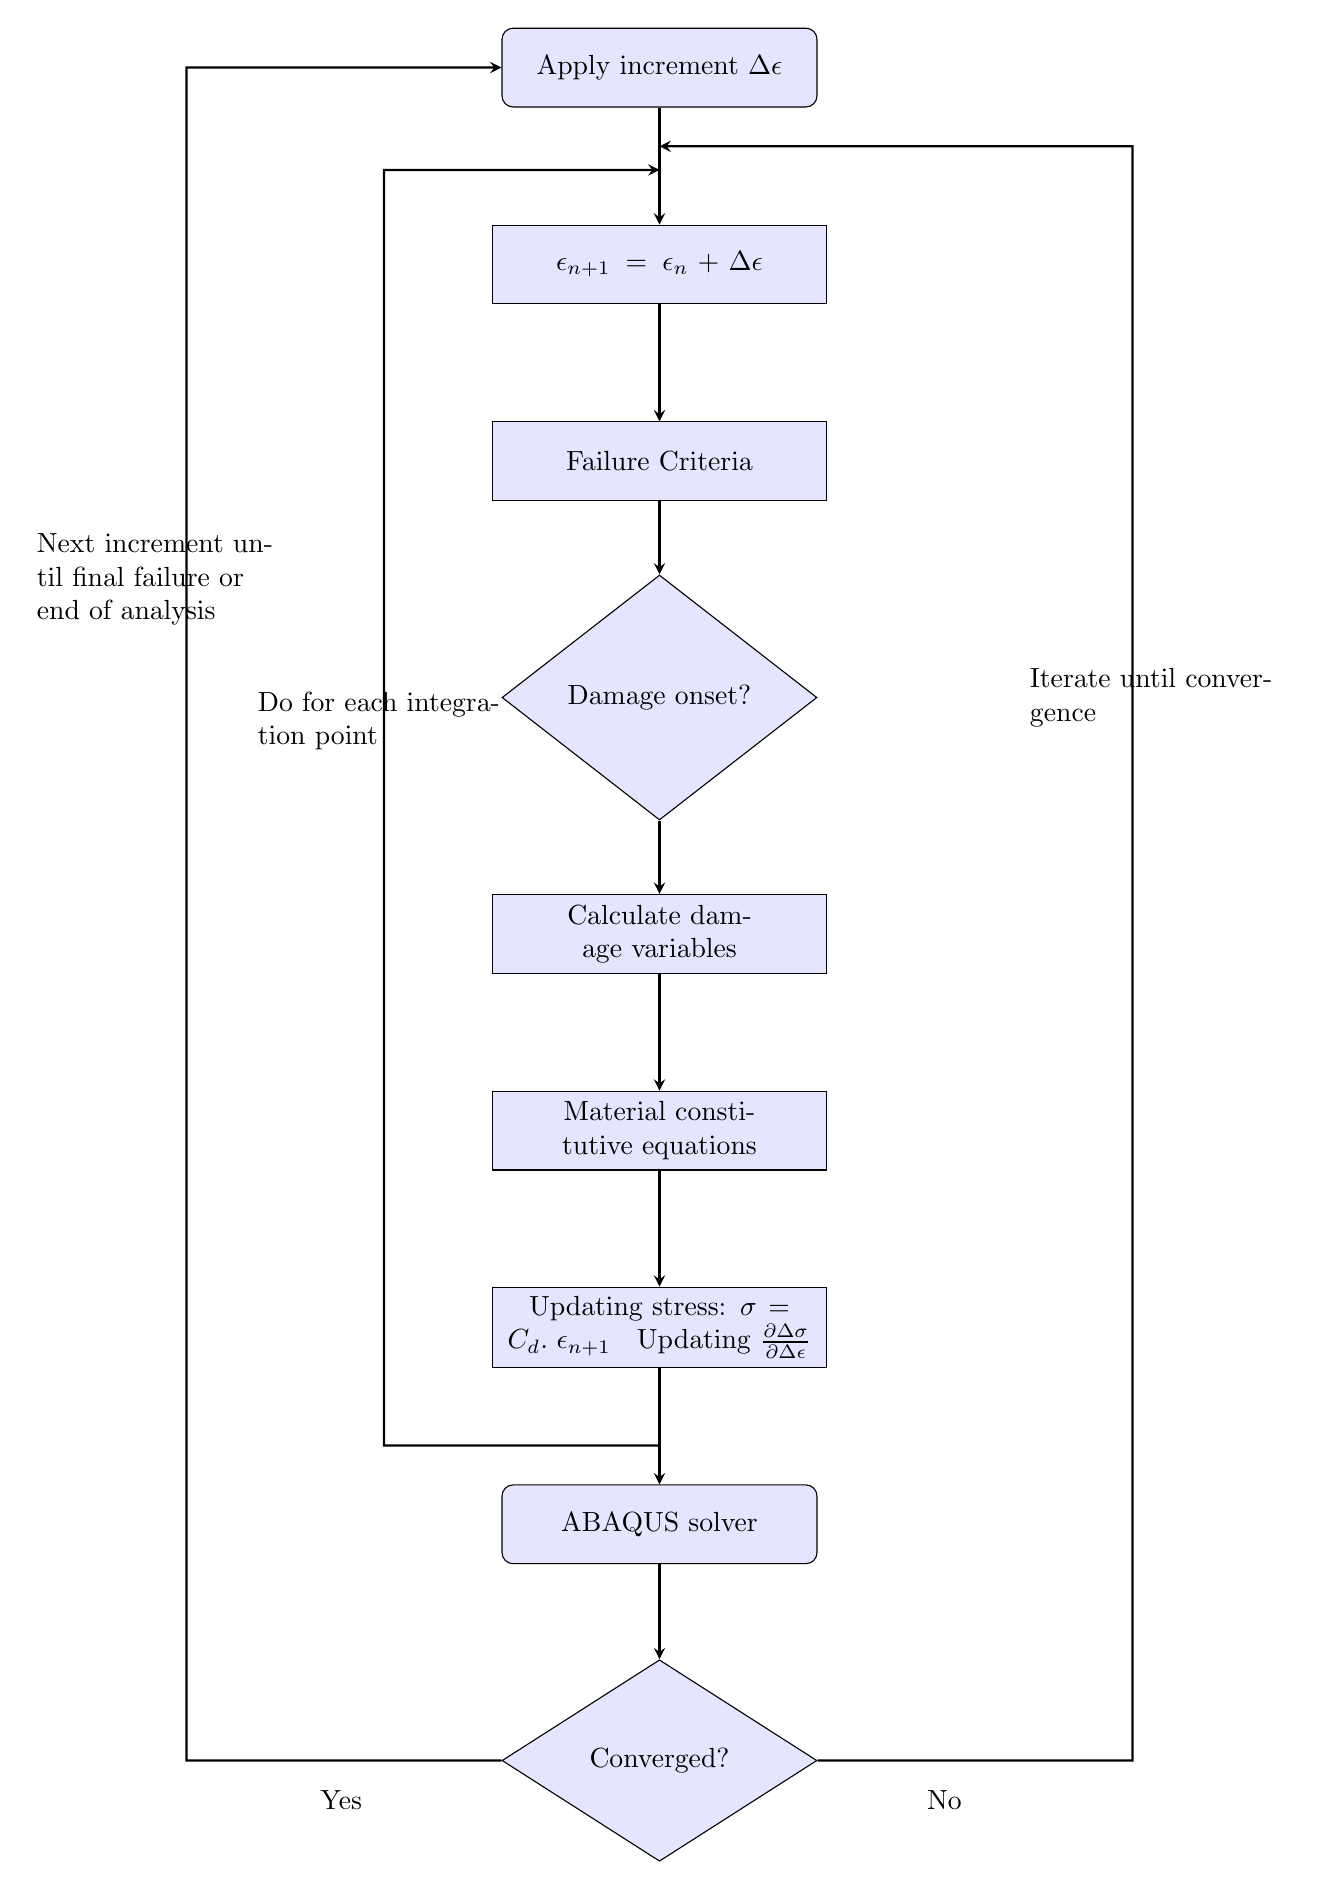
\begin{tikzpicture}[node distance = 2.5cm]

\node(straininc) [startstop] {Apply increment $\Delta\epsilon$};
\node(strainadd) [process, below of = straininc] {$\epsilon_{n+1} = \epsilon_{n} + \Delta\epsilon $};
\node(Failure)   [process, below of = strainadd] {Failure Criteria};
\node(Damageon)  [decision, below of = Failure, yshift = -0.5cm] {Damage onset?};
\node(Damagecalc) [process, below of = Damageon, yshift = -0.5cm] {Calculate damage variables};
\node(Materialeqn)[process, below of = Damagecalc] {Material constitutive equations};
\node(Tangent)[process, below of = Materialeqn] {Updating stress: $\sigma = C_{d}.\; \epsilon_{n + 1}$ \; Updating     $\frac{\partial \Delta \sigma}{\partial \Delta \epsilon}$};
\node(abaqus)[startstop, below of = Tangent] {ABAQUS solver};
\node(Converge)[decision, below of = abaqus, yshift = -0.5cm] {Converged?};

\draw [arrow] (straininc) -- (strainadd);
\draw [arrow] (strainadd) -- (Failure);
\draw [arrow] (Failure) -- (Damageon);
\draw [arrow] (Damageon) -- (Damagecalc);
\draw [arrow] (Damagecalc) -- (Materialeqn);
\draw [arrow] (Materialeqn) -- (Tangent);
\draw [arrow] (Tangent) -- (abaqus);
\draw [arrow] (abaqus) -- (Converge);
\draw [arrow] (Converge.west) -| ++(-4,2) -- ++(0,17.5) -- ++(0,2) --                
     node[xshift=-2.3cm,yshift=-6.5cm, text width=3.2cm]
     {Next increment until final failure or end of analysis}node[xshift=1.3cm,yshift=-22cm, text width=3.2cm]{Yes}(straininc.west);
\draw [arrow] (Converge.east) -| ++(4,2) -- ++(0,17.5) -- ++(0,1) --(0,-1)                
     node[near start,xshift=1.8cm,yshift=-7cm, text width=3.2cm]
     {Iterate until convergence}node[xshift=5cm,yshift=-21cm, text width=3.2cm]{No};
\draw [arrow] (0,-17.5)  -| ++(-3.5,0.7) -- ++(0,14.5) -- ++(0,1) -- (0,-1.3)               
     node[xshift=-3.5cm,yshift=-7cm, text width=3.2cm]
     {Do for each integration point};     
     
     

\end{tikzpicture}
\end{center}
\section{Constitutive damage model}
\indent\indent\indent  The thermodynamics of irreversible process is a general framework that can be used to formulate constitutive equations.  In order to establish a constitutive law, a scalar function corresponding to the complementary free energy density of the material has been defined. This function must be zero at the origin with respect to the free variables and must be positive definite. The proposed complementary free energy density for a damaged orthotropic lamina is given by

\begin{equation}
\psi = \frac{\sigma_{1}^{2}}{2(1 - d_{1})E_{1}} + \frac{\sigma_{2}^{2}}{2(1 - d_{2})E_{2}}  +  \frac{\nu_{12}}{E_{1}}\sigma_{1}\sigma_{2}  +  \frac{\sigma_{12}^{2}}{2(1 - d_{4})G_{12}} 
\end{equation}\\
where $E_{1}$,$G_{12}$, and $\nu_{12}$  are the Young's modulus, shear modulus and Poisson's ratio for the undamaged elastic material respectively. The damage variables $d_{1}$, $d_{2}$, and $d_{4}$ ensures that the composite ply maintains the original plane of material symmetry regardless of the damage state of the material. The variable $d_{1}$ is associated with the fibre failure, $d_{2}$  with the transverse matrix cracking and $d_{4}$ is influenced by longitudinal and transverse cracks. To ensure the thermodynamically irreversibility of the damage evolution, the rate of change of complementary free energy $\dot{G}$ minus the externally supplied work $\dot{\sigma}:\epsilon$, must not be negative:
\begin{equation}
\dot{G} - \dot{\sigma}:\epsilon  \geq 0
\end{equation}
This inequality describes the positiveness of the dissipated energy and has to be fulfilled by any constitutive model. Expanding the inequality in terms of damage variables and stress tensor gives
\begin{equation}
(\frac{\partial G}{\partial \sigma} - \epsilon) : \dot{\sigma} \; + \;\frac{\partial G}{\partial d_{1}}\dot{d_{1}}\; +\; \frac{\partial G}{\partial d_{2}}\dot{d_{2}}\; +\; \frac{\partial G}{\partial d_{6}}\dot{d_{6}}  \geq  0
\end{equation}
Since the stresses can vary freely, the expression in the parenthesis must be equal to zero to ensure the positive dissipation of mechanical energy. Therefore the strain tensor is first derivative of the complementary free energy density with respect to stress tensor.
\begin{equation}
\epsilon \; = \; \frac{\partial G}{\partial \sigma}  \; = \; H\;:\;\sigma
\end{equation}
Therefore the compliance tensor $H$ can be given as
$$
H \;=\;  \frac{\partial^{2} G}{\partial \sigma^{2}}\; =\;
 \begin{bmatrix}
  \frac{1}{(1 - d_{1})E_{1}}\; &\; -\frac{\nu_{21}}{E_{1}}\; &\; 0  \\
  \\
   -\frac{\nu_{12}}{E_{2}}\; &\; \frac{1}{(1 - d_{2})E_{2}}\; & \; 0  \\
   \\
  0\; &\; 0\; &\; \frac{1}{(1 - d_{6})G_{12}} 
 
 \end{bmatrix}
 $$
The complementary free energy density for a 3D case is given by
\begin{equation}
\psi \;=\; \frac{\sigma_{1}^{2}}{2(1 - d_{1})E_{1}} + \frac{\sigma_{2}^{2}}{2(1 - d_{2})E_{2}}\;  + \; \frac{\sigma_{3}^{2}}{2(1 - d_{3})E_{3}}\; + \; \frac{\nu_{12}}{E_{1}}\sigma_{1}\sigma_{2}\; +\; \frac{\nu_{13}}{E_{1}}\sigma_{1}\sigma_{3} \; +\; 
\end{equation}
\begin{align*}
\frac{\nu_{23}}{E_{2}}\sigma_{2}\sigma_{3}\; + \; \frac{\sigma_{12}^{2}}{2(1 - d_{4})G_{12}}\; + \; \frac{\sigma_{23}^{2}}{2(1 - d_{5})G_{23}}\; +  \; \frac{\sigma_{13}^{2}}{2(1 - d_{6})G_{13}}
\end{align*}
\newpage
The compliance tensor $H$ for 3D case can be given as
$$
H \; = \; 
 \begin{bmatrix}
  \frac{1}{(1 - d_{1})E_{1}} & -\frac{\nu_{12}}{E_{1}} & -\frac{\nu_{13}}{E_{1}} & 0 & 0 & 0 \\
  \\
  -\frac{\nu_{21}}{E_{2}} & \frac{1}{(1 - d_{2})E_{2}} & -\frac{\nu_{23}}{E_{2}} & 0 & 0 & 0 \\
	\\  
  -\frac{\nu_{31}}{E_{3}} & -\frac{\nu_{32}}{E_{3}} & \frac{1}{(1 - d_{3})E_{3}} & 0 & 0 & 0 \\
  \\
  0 & 0 & 0 & \frac{1}{(1 - d_{4})G_{12}} & 0 & 0 \\
  \\
  0 & 0 & 0 & 0 & \frac{1}{(1 - d_{5})G_{23}} & 0 \\
  \\
  0& 0 & 0 & 0 & 0 & \frac{1}{(1 - d_{5})G_{13}} 
 \end{bmatrix}
 $$
\subsection{Damage activation functions}
\indent\indent\indent Damage activation function(DAF) defines the elastic domain with in which the material is linearly elastic. The determination of the domain of elastic response under stress states is an essential component of accurate damage model. The DAF can be defined as
\begin{equation}
g_{m} \; = \; \hat{g_{m}} \; - \; \hat{\gamma_{m}}  \leq  0
\end{equation} 
where $\hat{g_{m}}$ is the positive loading function that depends on stress states and $\hat{\gamma_{m}}$ is the updated threshold function and $m$ refers to the failure mode.
\newpage
\section{Three dimensional Continuum damage mechanics model}
\indent\indent\indent A symmetric second order tensor D, has been chosen as the damage tensor and its principal directions are assumed to coincide with the principal material directions. The $i^{th}$ eigen value $d_{i}$ represents the effective fractional reduction in load carrying area on planes that are perpendicular to the $i^{th}$ principal material direction. The first principal direction coincides with the fiber direction and the second and the third material direction are made to coincide with the transverse and ply stacking direction. The eigen value of the damage tensor must be in the range $0 \leq d_{i} \leq  1  $, where $d_{i}$ = 0 means complete lack of microcracks in the $i^{th}$ principal material direction, while $d_{i}$ = 1 means complete separation of material across the planes that are normal to the $i^{th}$ principal material direction.

$$
D \; = \; 
 \begin{bmatrix}
  d_{1} & 0 & 0  \\
  \\
  0 & d_{2} & 0  \\
  \\  
  0 & 0 & d_{3} \\
  
 \end{bmatrix}
 $$  
 
The effective stress tensor can be defined as 
\begin{equation}
   \bar{\sigma} \; = \; M(D) : \sigma
\end{equation}  
where
\begin{equation*}
M(D) \; = \; diag\;[1/\omega_{11}\;\;1/\omega_{22}\;\;1/\omega_{33}\;\;1/\omega_{12}\;\;1/\omega_{13}\;\;1/\omega_{23}\;]
\end{equation*}
\begin{equation*}
\omega_{11}\; = \; 1 - d_{1}, \;\; \omega_{22}\; = \; 1 - d_{2}, \;\;\omega_{33}\; = \; 1 - d_{3} \;\; \omega_{12}\; = \; \sqrt{(1 - d_{1})(1 - d_{2})} \;\;
\end{equation*}
\begin{equation*}
 \omega_{13}\; = \; \sqrt{(1 - d_{1})(1 - d_{3})} \;\;  \omega_{23}\; = \; \sqrt{(1 - d_{2})(1 - d_{3})} \;\;
\end{equation*}
The effective stress is introduced into the strain energy equivalence principle. The strain energy of the material without damage can be expressed as 
\begin{equation}
W = \frac{1}{2}\sigma:C^{-1}:\sigma
\end{equation}
The equivalence of strain energy for damaged material is given by
\begin{equation}
W^{d} = \frac{1}{2}\bar{\sigma}:C^{-1}:\bar{\sigma} \; = \; \frac{1}{2}\sigma: M^{T}:C^{-1}:M:\sigma
\end{equation}
So the strain can be calculated as follows
\begin{equation}
\epsilon = \frac{\partial W^{d}}{\partial \sigma} = (M^{T}:C^{-1}:M):\sigma
\end{equation}
The constitutive equation of the damaged composite laminates is given as 
\begin{equation}
C^{d}\; = \; M^{-1}:C:M^{T,-1}
\end{equation}
\newpage
The stiffness matrix of the damaged composite lamina in matrix form can be represented as follows
\begin{tiny}
\begin{equation*}
C^{d} \; = \; 
 \begin{bmatrix}
  C_{11}(1 - d_{1})^{2} & C_{12}(1 - d_{1})(1 - d_{2}) & C_{13}(1 - d_{1})(1 - d_{3})  & 0 & 0 & 0 \\
  \\
  C_{21}(1 - d_{2})(1 - d_{1}) & C_{22}(1 - d_{2})^{2}  & C_{23}(1 - d_{2})(1 - d_{3}) & 0 & 0 & 0 \\
 \\  
  C_{31}(1 - d_{3})(1 - d_{1}) & C_{32}(1 - d_{3})(1 - d_{2}) & C_{33}(1 - d_{3})^{2}  & 0 & 0 & 0 \\
  \\
  0 & 0 & 0 & C_{44}(1 - d_{1})(1 - d_{2})   & 0 & 0 \\
  \\
  0 & 0 & 0 & 0 & C_{55}(1 - d_{1})(1 - d_{3}) & 0 \\
  \\
  0& 0 & 0 & 0 & 0 & C_{66}(1 - d_{2})(1 - d_{3}) 
 \end{bmatrix}
\end{equation*}
\end{tiny}

 
\end{document}